\documentclass{article}
\usepackage{amsmath}
\usepackage{tikz}

\begin{document}

Sea $G = (E,V)$ un grafo, con $P$ y $Q$ dos caminos distintos que nos llevan de $v$ a $w$. Los notamos:
\[ P = v_0, \ldots, v_p \quad \text{y} \quad Q = w_0, \ldots, w_q \quad \text{con} \quad v_0 = w_0 = v \quad \text{y} \quad v_p = w_q = w \]

Observemos:

\begin{enumerate}
    \item Si $P$ y $Q$ no comparten ningún vértice intermedio, entonces podemos generar un ciclo que va desde $v$ hasta $w$ por $Q$. Luego desde $w$, podemos volver a $v$ a través de $P$, generándonos un ciclo. Por ejemplo:
    \begin{center}
    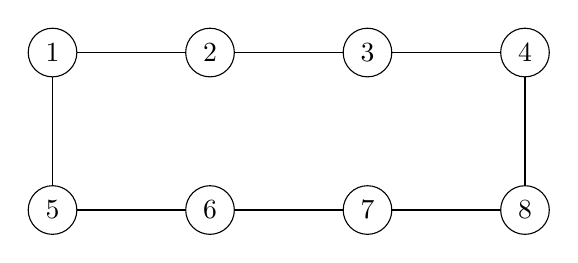
\begin{tikzpicture}
      \node[circle,draw] (1) at (0,0) {1};
      \node[circle,draw] (2) at (2,0) {2};
      \node[circle,draw] (3) at (4,0) {3};
      \node[circle,draw] (4) at (6,0) {4};
      \node[circle,draw] (5) at (0,-2) {5};
      \node[circle,draw] (6) at (2,-2) {6};
      \node[circle,draw] (7) at (4,-2) {7};
      \node[circle,draw] (8) at (6,-2) {8};
      \draw (1) -- (2);
      \draw (2) -- (3);
      \draw (3) -- (4);
      \draw (1) -- (5);
      \draw (5) -- (6);
      \draw (6) -- (7);
      \draw (7) -- (8);
      \draw (4) -- (8);
    \end{tikzpicture}
    \end{center}
    Aquí, $P = 1,2,3,4$ y $Q = 1,5,6,4$.
    
    \item Si $P$ y $Q$ comparten algún vértice intermedio, tenemos dos casos:
    \begin{enumerate}
        \item Si solo comparten un vértice intermedio, podemos generar el ciclo desde $v_0$ hasta $x$ y luego desde $x$ hasta $q_0$. Generándonos así un ciclo. Por ejemplo:
        \begin{center}
        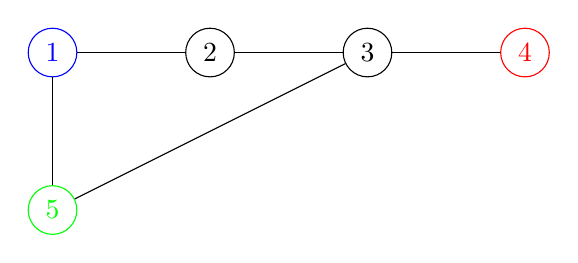
\begin{tikzpicture}
          \node[circle,draw,blue] (1) at (0,0) {1};
          \node[circle,draw] (2) at (2,0) {2};
          \node[circle,draw] (3) at (4,0) {3};
          \node[circle,draw,red] (4) at (6,0) {4};
          \node[circle,draw,green] (5) at (0,-2) {5};
          \draw (1) -- (2);
          \draw (2) -- (3);
          \draw (3) -- (4);
          \draw (1) -- (5);
          \draw (5) -- (3);
        \end{tikzpicture}
        \end{center}
        Aquí, $P = 1,2,3,4$ y $Q = 1,5,3,4$.
        
        \item Si comparten más de un vértice intermedio, podemos tomar dos $x$ y $x'$ y generar un ciclo entre ellos. Por ejemplo:
        \begin{center}
        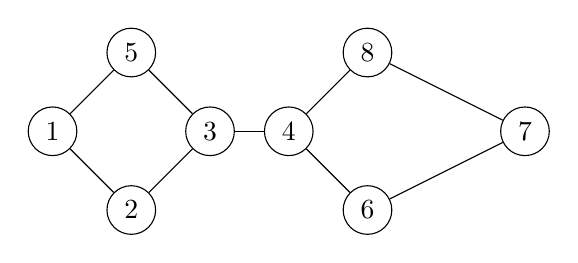
\begin{tikzpicture}
          \node[circle,draw] (1) at (0,-1) {1};
          \node[circle,draw] (2) at (1,-2) {2};
          \node[circle,draw] (3) at (2,-1) {3};
          \node[circle,draw] (4) at (3,-1) {4};
          \node[circle,draw] (5) at (1,0) {5};
          \node[circle,draw] (6) at (4,-2) {6};
          \node[circle,draw] (7) at (6,-1) {7};
          \node[circle,draw] (8) at (4,0) {8};
          \draw (1) -- (2);
          \draw (2) -- (3);
          \draw (3) -- (4);
          \draw (4) -- (6);
          \draw (3) -- (5);
          \draw (1) -- (5);          
          \draw (4) -- (8);
          
          \draw (6) -- (7);
          \draw (7) -- (8);
        \end{tikzpicture}
        \end{center}
        Aquí, $P = 1,2,3,4,8,7$ y $Q = 1,5,3,4,6,7$.
    \end{enumerate}
\end{enumerate}
\newpage
Ahora la demostración:

Sea $G = (E,V)$ un grafo, con $P$ y $Q$ dos caminos distintos que nos llevan de $v$ a $w$, tal que $G$ no tenga ningún ciclo que contenga vértices de $P$ o $Q$.

Los notamos: 
\[ P = v_0, \ldots, v_p \quad \text{y} \quad Q = w_0, \ldots, w_q \quad \text{con} \quad v_0 = w_0 = v \quad \text{y} \quad v_p = w_q = w \]

Como $P$ y $Q$ son distintos, deben tener al menos un vértice distinto, formalmente:
\[ \exists v \in P \land v \notin Q \quad \lor \quad \exists v \in Q \land v \notin P \]

Supongamos que ningún vértice de $P$ o $Q$ pertenece al ciclo, entonces debe existir al menos un vértice $v'$ distinto del origen y el final ($v' \neq v_0 \neq w_0$ y $v' \neq v_p \neq w_q$) que pertenezca tanto a $P$ como a $Q$ (de otra forma $P$ y $Q$ formarían un ciclo). Llamémoslo $v'$ que cumple $v' \in P \land v' \in Q$.

Ahora podemos definir $P' = (v',v'_1 , \ldots , v_p)$ y $Q' = (v',w'_1, \ldots , w'_q)$. Claramente $P' \subseteq P$ y $Q' \subseteq Q$.\\

¿Y ahora? Si los caminos son del todo distintos, entonces tenemos ya nuestro ciclo, pero como dijimos que $G$ no contiene un ciclo con elementos de $P$ y $Q$, podemos repetir la operación anterior. Es decir, debe existir un elemento $v''$ que $P'$ y $Q'$ compartan, distinto del principio y el final, y repetimos.\\

¿Hasta cuántas veces podremos hacer esto? La cantidad máxima es $\min(|P|,|Q|)$, dado que (por hipótesis) ningún ciclo se puede formar con elementos de $P$ y $Q$, entonces la única manera que esto se cumpla cada vez, es que $P$ sea igual a $Q$; pero esto es absurdo, ya que dijimos que $P$ es distinto de $Q$ por al menos un vértice.

Luego, dados $P$ y $Q$ en $G$, que cumplan todo lo pedido, debe existir un ciclo con elementos de $P$ o elementos de $Q$.


\end{document}
